\documentclass{sephdthesis}
\usepackage{graphicx}
\usepackage[unicode]{hyperref}
\usepackage{multirow}
\let\newfloat\undefined
\usepackage[capbesideposition={top,inside},facing=yes,capbesidesep=quad]{floatrow}
\newfloatcommand{tcapside}{table}[\capbeside]

\captionnamefont{\bfseries}

\address{SE-221 00 LUND}
\author{The author name}
\country{Some country}
\covertext{Explanation of the cover figure.} % Leave empty if none.
\date{A year}
\defenddate{Defence data}
\defendplace{Defence room}
\degree{The degree}
%\degreetitle{MD}
\department{The department}
%\disseries{Dissertation series} % Comment out if none
\email{The email address} % Comment out if none
\faculty{The faculty}
%\fulltext{http://theses.lub.lu.se/postgrad} % Where to find electronic full text, comment out if none.
\institution{The university}
\isbn{ISBN ???--??--????--???--?}
\issn{ISSN ????--????}
\logotype{figures/university_logo}
\opponent{The name of the opponent}
\printer{The printer}
\subtitle{The subtitle}
\thesistype{Thesis type}
\title{Title of the thesis}
\shorttitle{\thetitle}
%\webaddress{http://some_domain.root} % Comment out if none

%%%%% Definitions

%\hyphenation{}

\endinput


\begin{document}
%\layout
%---------
\frontmatter \maketitle
%---------
\thispagestyle{cleared}
\hbox{}\vfill
\begin{flushright}
\begin{minipage}[l]{0.6\textwidth}
	Some quote.
  \emph{--Said by someone}
  \end{minipage}
\end{flushright}

\vspace{4cm}
\endinput
\cleardoublepage
%---------
\tableofcontents\cleardoublepage
%---------
\chapter{List of original papers}
\renewcommand{\theenumi}{\Roman{enumi}}
This thesis is based on the following papers, which in the text will
be referred to by their Roman numerals.

\begin{enumerate}
\raggedright \setlength{\parindent}{0pt}
\item Lorem ipsum dolor sit amet, consectetur adipiscing elit. Morbi suscipit est a nunc luctus, eget lobortis nunc porttitor. Nam sit amet leo gravida, pulvinar ligula sed, maximus nibh. Ut vel.
\item Lorem ipsum dolor sit amet, consectetur adipiscing elit. Morbi suscipit est a nunc luctus, eget lobortis nunc porttitor. Nam sit amet leo gravida, pulvinar ligula sed, maximus nibh. Ut vel.
\item Lorem ipsum dolor sit amet, consectetur adipiscing elit. Morbi suscipit est a nunc luctus, eget lobortis nunc porttitor. Nam sit amet leo gravida, pulvinar ligula sed, maximus nibh. Ut vel.
\end{enumerate}
\renewcommand{\theenumi}{\arabic{enumi}}
\cleardoublepage
%---------
\chapter{Abstract}
Lorem ipsum dolor sit amet, consectetur adipiscing elit. Duis vitae efficitur ligula, ac malesuada arcu. Cras sed vehicula eros, id pharetra odio. Aenean eu lacinia mauris. Integer ex leo, consectetur ut tempor in, dapibus in ligula. Donec a nunc et ex faucibus laoreet et eu lacus. Nulla vel odio nec massa feugiat molestie vitae sed nisi. Ut sed scelerisque mi.

Pellentesque sapien tellus, iaculis et neque id, sagittis suscipit ex. Aliquam at rhoncus quam. Morbi sed egestas erat, id rhoncus elit. Pellentesque quis velit libero. Nulla porta arcu viverra metus tincidunt, in volutpat urna tristique. Curabitur sit amet odio velit. Maecenas ullamcorper tellus ipsum, ut fringilla erat maximus a. Duis massa orci, ultrices vel eros at, eleifend pharetra purus. Sed lobortis sagittis facilisis.\cleardoublepage
%---------
\chapter{Populärvetenskaplig sammanfattning}
\begin{otherlanguage}{swedish}
Lorem ipsum dolor sit amet, consectetur adipiscing elit. Duis vitae efficitur ligula, ac malesuada arcu. Cras sed vehicula eros, id pharetra odio. Aenean eu lacinia mauris. Integer ex leo, consectetur ut tempor in, dapibus in ligula. Donec a nunc et ex faucibus laoreet et eu lacus. Nulla vel odio nec massa feugiat molestie vitae sed nisi. Ut sed scelerisque mi.

Pellentesque sapien tellus, iaculis et neque id, sagittis suscipit ex. Aliquam at rhoncus quam. Morbi sed egestas erat, id rhoncus elit. Pellentesque quis velit libero. Nulla porta arcu viverra metus tincidunt, in volutpat urna tristique. Curabitur sit amet odio velit. Maecenas ullamcorper tellus ipsum, ut fringilla erat maximus a. Duis massa orci, ultrices vel eros at, eleifend pharetra purus. Sed lobortis sagittis facilisis.

\end{otherlanguage}
\cleardoublepage
%---------
\chapter{Abbreviations}

\begin{tabular}{ll}
\multicolumn{2}{l}{\textbf{Technical terms}}\\
\toprule\\
???? & Pellentesque sapien tellus, iaculis et neque id.\\
???? & Pellentesque sapien tellus, iaculis et neque id \\
???? & Pellentesque sapien tellus, iaculis et neque id\\
\bottomrule
\\
\multicolumn{2}{l}{\textbf{Organisations}}\\
\toprule\\
???? & Pellentesque sapien tellus, iaculis et neque id. \\
???? & Pellentesque sapien tellus, iaculis et neque id. \\
\bottomrule
\end{tabular}

\cleardoublepage
%---------
\mainmatter% \chapterheadings
\pagestyle{ruled}
\nouppercaseheads
%---------
\chapter{Introduction}
\section{Historical background}
Lorem ipsum dolor sit amet, consectetur adipiscing elit. Duis vitae efficitur ligula, ac malesuada arcu. Cras sed vehicula eros, id pharetra odio. Aenean eu lacinia mauris. Integer ex leo, consectetur ut tempor in, dapibus in ligula. Donec a nunc et ex faucibus laoreet et eu lacus. Nulla vel odio nec massa feugiat molestie vitae sed nisi. Ut sed scelerisque mi.

Pellentesque sapien tellus, iaculis et neque id, sagittis suscipit ex. Aliquam at rhoncus quam. Morbi sed egestas erat, id rhoncus elit. Pellentesque quis velit libero. Nulla porta arcu viverra metus tincidunt, in volutpat urna tristique. Curabitur sit amet odio velit. Maecenas ullamcorper tellus ipsum, ut fringilla erat maximus a. Duis massa orci, ultrices vel eros at, eleifend pharetra purus. Sed lobortis sagittis facilisis.
\cleardoublepage
%---------
\chapter{Theory}
\section{Section}
\subsection{Sub-section}
Lorem ipsum dolor sit amet, consectetur adipiscing elit Table~\ref{tab:table_2}. Duis vitae efficitur ligula, ac malesuada arcu. Cras sed vehicula eros, id pharetra odio. Aenean eu lacinia mauris. Integer ex leo, consectetur ut tempor in, dapibus in ligula. Donec a nunc et ex faucibus laoreet et eu lacus. Nulla vel odio nec massa feugiat molestie vitae sed nisi. Ut sed scelerisque mi.

Pellentesque sapien tellus, iaculis et neque id, sagittis suscipit ex. Aliquam at rhoncus quam. Morbi sed egestas erat, id rhoncus elit. Pellentesque quis velit libero. Nulla porta arcu viverra metus tincidunt, in volutpat urna tristique. Curabitur sit amet odio velit. Maecenas ullamcorper tellus ipsum, ut fringilla erat maximus a. Duis massa orci, ultrices vel eros at, eleifend pharetra purus. Sed lobortis sagittis facilisis \cite{Long:2007uv}.

\begin{table}
	\tcapside
	{\caption{Caption of table with side caption.}\label{tab:table_2}}
	{\begin{tabular}{rcc}
		\toprule
		& Bkg. & Bkg. \\
		& high & low \\
		\midrule
		Speed fast & \multirow{2}{*}{Short} & \multirow{2}{*}{Long} \\
		Dist. long & & \\
		\midrule
		Speed fast & Very & \multirow{2}{*}{Short} \\
		Dist. short & short & \\
		\midrule
		Speed slow & \multirow{2}{*}{Long} & Very \\
		Dist. long &  & long \\
		\midrule
		Speed slow & \multirow{2}{*}{Short} & \multirow{2}{*}{Long} \\
		Dist. short & & \\
		\bottomrule
	\end{tabular}}
\end{table}
\cleardoublepage
%---------
\chapter{Materials and methods}
\section{Section}
Lorem ipsum dolor sit amet, consectetur adipiscing elit Table~\ref{tab:table_1}. Duis vitae efficitur ligula, ac malesuada arcu. Cras sed vehicula eros, id pharetra odio. Aenean eu lacinia mauris. Integer ex leo, consectetur ut tempor in, dapibus in ligula. Donec a nunc et ex faucibus laoreet et eu lacus. Nulla vel odio nec massa feugiat molestie vitae sed nisi. Ut sed scelerisque mi.

\subsection{Subsection}
Pellentesque sapien tellus, iaculis et neque id, sagittis suscipit ex. Aliquam at rhoncus quam. Morbi sed egestas erat, id rhoncus elit. Pellentesque quis velit libero. Nulla porta arcu viverra metus tincidunt, in volutpat urna tristique. Curabitur sit amet odio velit. Maecenas ullamcorper tellus ipsum, ut fringilla erat maximus a. Duis massa orci, ultrices vel eros at, eleifend pharetra purus. Sed lobortis sagittis facilisis \cite{Tyler:1996ur}.

\begin{table}
	\ttabbox
	{\caption{Caption of regular table.}\label{tab:table_1}}
	{\begin{minipage}{\textwidth}\begin{tabular}{lcccc}
		\toprule
		& \multicolumn{4}{c}{Detector system} \\
		& \cline{1-4}
		& \multicolumn{1}{c}{1} & \multicolumn{1}{c}{2} & \multicolumn{1}{c}{3} & \multicolumn{1}{c}{4}\\
		\midrule
		Type	            	 			& HPGe 		& NaI 	& NaI 	& LaBr  \\
		Volume (l)          				& 0.48 		& 0.35 		& 4 		& 0.35 \\
		Efficiency (\%) 		& 123	  	& 100  		& n/a  		& 135  \\
		Resolution\footnote{FWHM of the 662~keV Cs-137 peak.} (\%) 					& 0.15 		& 7.5  		& 7.5 		& 3.0   \\
		Electronics 						& DigiDART 	& DigiBASE 	& DigiBASE 	& DigiBASE \\
		Used in paper						& I, II, IV	& I, II, V 	& III 		& II \\
		\bottomrule
	\end{tabular}\end{minipage}}
\end{table}\cleardoublepage
%---------
\chapter{Results and discussion}
\section{Section 1}
Lorem ipsum dolor sit amet, consectetur adipiscing elit Figure~\ref{fig:figure_1}. Duis vitae efficitur ligula, ac malesuada arcu. Cras sed vehicula eros, id pharetra odio. Aenean eu lacinia mauris. Integer ex leo, consectetur ut tempor in, dapibus in ligula. Donec a nunc et ex faucibus laoreet et eu lacus. Nulla vel odio nec massa feugiat molestie vitae sed nisi. Ut sed scelerisque mi.

Pellentesque sapien tellus, iaculis et neque id, sagittis suscipit ex. Aliquam at rhoncus quam. Morbi sed egestas erat, id rhoncus elit. Pellentesque quis velit libero. Nulla porta arcu viverra metus tincidunt, in volutpat urna tristique. Curabitur sit amet odio velit. Maecenas ullamcorper tellus ipsum, ut fringilla erat maximus a. Duis massa orci, ultrices vel eros at, eleifend pharetra purus. Sed lobortis sagittis facilisis.

\begin{figure}
	\fcapside
	{\caption{Figure with side caption.}\label{fig:figure_1}}
	{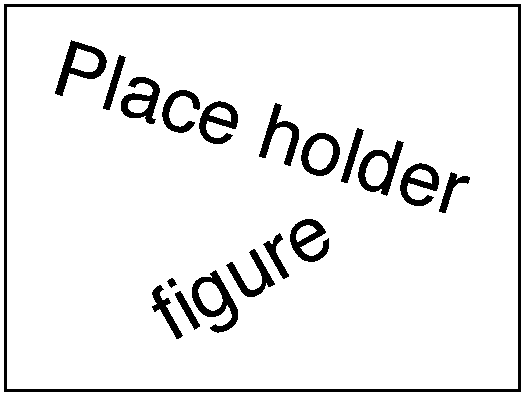
\includegraphics[width=0.5\linewidth]{figures/results/place_holder}}
\end{figure}

\section{Section 2}
Lorem ipsum dolor sit amet, consectetur adipiscing elit Figure~\ref{fig:figure_2}. Nunc luctus risus ac dapibus finibus. Ut eu volutpat purus. Nunc elit mi, tincidunt at sodales ut, pulvinar nec neque. Phasellus gravida ullamcorper ante, sit amet varius diam feugiat id. Fusce vestibulum, mauris id egestas varius, augue velit posuere odio, et pellentesque elit velit at dolor. Praesent ac mi eros. Ut sed vulputate magna, quis mattis ipsum. Praesent mauris sapien, tincidunt et enim vitae, vulputate ornare lorem. Cras egestas, neque ut condimentum bibendum, ligula lorem bibendum tortor, vitae finibus odio metus quis lectus. Duis sit amet ultricies odio. Vestibulum ante ipsum primis in faucibus orci luctus et ultrices posuere cubilia Curae; Sed eleifend cursus ex et faucibus. Proin imperdiet sodales diam, sed varius eros cursus non. Donec ex massa, aliquet ultricies laoreet et, dignissim eget diam. Suspendisse ut tincidunt neque.

\begin{figure}
	\ffigbox
	{\caption{Figure with regular caption.}\label{fig:figure_2}}
	{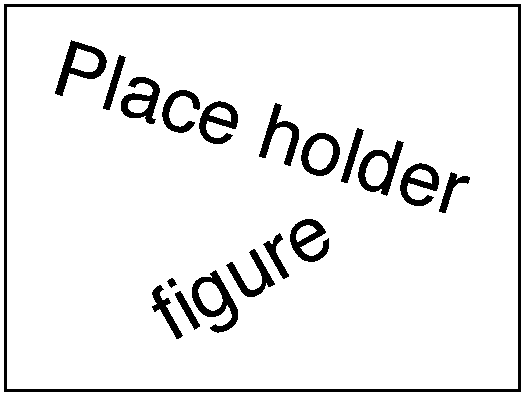
\includegraphics[width=\linewidth]{figures/results/place_holder}}
\end{figure}

Donec vitae congue turpis. Morbi maximus ligula eu nunc ultrices ultricies. Donec porta libero lacus, quis mollis enim vestibulum eget. Phasellus mollis blandit fringilla. Duis a mauris eleifend, rutrum nisl eget, mollis mauris. Donec eget orci et nunc condimentum dapibus. Quisque fermentum cursus pellentesque. Maecenas vel ante malesuada, tempus quam in, pulvinar augue. Ut at dui erat. Quisque non erat a sapien vestibulum euismod ac quis augue. Donec velit turpis, sollicitudin eu risus sed, fringilla bibendum orci. Vivamus tempus dolor a odio tincidunt vulputate. In tristique nisi nibh, sit amet accumsan arcu tincidunt et. Interdum et malesuada fames ac ante ipsum primis in faucibus. Pellentesque suscipit urna sit amet libero finibus convallis. Praesent sodales lacinia velit et tincidunt.

Curabitur ultrices augue erat, in aliquam urna faucibus a. Phasellus eu mattis nisi, accumsan eleifend tortor. Donec eget scelerisque velit. Ut aliquet mauris tristique nisl hendrerit, eget interdum justo venenatis. Phasellus ac euismod turpis. Phasellus a nisl ut enim ultrices varius sollicitudin ut augue. Sed eu justo efficitur, ornare nibh eu, semper lectus \cite{Geelhood:1998vs}.\cleardoublepage
%---------
\chapter{Major conclusions}
\renewcommand{\theenumi}{\Roman{enumi}}
Lorem ipsum dolor sit amet, consectetur adipiscing elit. Duis vitae efficitur ligula, ac malesuada arcu. Cras sed vehicula eros, id pharetra odio. Aenean eu lacinia mauris. Integer ex leo, consectetur ut tempor in, dapibus in ligula. Donec a nunc et ex faucibus laoreet et eu lacus. Nulla vel odio nec massa feugiat molestie vitae sed nisi. Ut sed scelerisque mi.

Pellentesque sapien tellus, iaculis et neque id, sagittis suscipit ex. Aliquam at rhoncus quam. Morbi sed egestas erat, id rhoncus elit. Pellentesque quis velit libero. Nulla porta arcu viverra metus tincidunt, in volutpat urna tristique. Curabitur sit amet odio velit. Maecenas ullamcorper tellus ipsum, ut fringilla erat maximus a. Duis massa orci, ultrices vel eros at, eleifend pharetra purus. Sed lobortis sagittis facilisis.

The major conclusion of each paper were as follows:
\begin{enumerate}
	\item Lorem ipsum dolor sit amet, consectetur adipiscing elit. Duis vitae efficitur ligula, ac malesuada arcu. Cras sed vehicula eros, id pharetra odio. Aenean eu lacinia mauris. Integer ex leo, consectetur ut tempor in, dapibus in ligula. Donec a nunc et ex faucibus laoreet et eu lacus. Nulla vel odio nec massa feugiat molestie vitae sed nisi. Ut sed scelerisque mi.

	\item Pellentesque sapien tellus, iaculis et neque id, sagittis suscipit ex. Aliquam at rhoncus quam. Morbi sed egestas erat, id rhoncus elit. Pellentesque quis velit libero. Nulla porta arcu viverra metus tincidunt, in volutpat urna tristique. Curabitur sit amet odio velit. Maecenas ullamcorper tellus ipsum, ut fringilla erat maximus a. Duis massa orci, ultrices vel eros at, eleifend pharetra purus. Sed lobortis sagittis facilisis.
\end{enumerate}

\renewcommand{\theenumi}{\arabic{enumi}}\cleardoublepage
%---------
\backmatter
\chapter{Acknowledgments}
Lorem ipsum dolor sit amet, consectetur adipiscing elit. Pellentesque placerat arcu velit, sit amet pellentesque dolor maximus ut. Pellentesque eu gravida lectus, vitae facilisis diam. Pellentesque vitae facilisis tellus. Nullam sit amet turpis posuere, convallis ante ut, pellentesque neque. Fusce tincidunt nisl eget diam iaculis sagittis. Maecenas quis quam id nunc posuere fermentum a vitae urna. Nullam rhoncus dolor vitae turpis porta, non cursus velit accumsan. Mauris convallis blandit ligula, pretium varius leo dapibus vitae. Praesent sed magna orci. Proin scelerisque est sit amet nunc scelerisque sollicitudin. Vestibulum dignissim maximus neque. Fusce vitae eros dictum, lacinia dolor a, luctus diam. Quisque convallis quis nulla eu dignissim. Pellentesque eu scelerisque mauris. Maecenas nec nunc et enim consectetur iaculis vel at mauris.

Aenean mollis, nulla sit amet vulputate tincidunt, enim augue tempus purus, ut lobortis velit augue sed nisl. Vestibulum venenatis maximus leo, id commodo nunc malesuada vel. Nulla sem lectus, efficitur eu orci id, porta auctor dolor. Duis venenatis ut arcu vel faucibus. In ut elit vel sem interdum aliquam eu a tortor. In vel tincidunt ante. Praesent nec viverra dolor. Nulla orci ligula, blandit sit amet ex non, commodo sollicitudin ex. Maecenas ac posuere nunc.\cleardoublepage

\pagestyle{bib_style}
\bibliographystyle{ieeetr}
\bibliography{phd_papers}

\cftaddtitleline{toc}{chapter}{Papers I-V}{}

\end{document}
